\section{Linear and kernel models}
\subsection{MLR}
\begin{frame}[t]{Multiple linear regression}
Linear models give $\hat{y}$ as linear function of the data matrix of $X$:
\begin{align*}
&\hat{y}_{MLR}(x^{*}) = \sum_{j=1}^{d} w_j x^{*}_j  +w_{0} \visible<2->{= \begin{bmatrix}  1 & x^{*}_1 & \hdots & x^{*}_d  \end{bmatrix} \begin{bmatrix} w_0 \\ w_1 \\ \vdots \\ w_d  \end{bmatrix} }
\end{align*}
\visible<3->{We can write this in a matrix form as well:
\begin{align*}
    &\hat{y}_{MLR}(X) = \begin{bmatrix}  1 &  x^{(1)}_{1} & x^{(1)}_{2} & \hdots x^{(1)}_{d}  \\  \vdots  &&&\vdots \\  1&  x^{(n)}_{1} & x^{(n)}_{2} & \hdots x^{(n)}_{d} \end{bmatrix} w  = X'w\\
\end{align*}
}
\visible<4->{Notice how we handle the constant terms} 
\end{frame}
\begin{frame}[t]{Multiple linear regression II}


Consider our objective:
\begin{align*}
w =& \arg \min_{ w \in \mathbb{R}^{p}} \left\Vert y_{data}-Xw \right\Vert^2 + \lambda\left\Vert w\right\Vert^{2} \\
\implies & -2X^T\left(y_{data} - Xw\right) + 2\lambda w = 0\\
& \uncover<2->{(\lambda I + X^TX )w = X^Ty_{data}} \\
&  \uncover<3->{ w = \left(\lambda I + X^TX\right)^{-1} X^Ty_{data}}
\end{align*}
For any positive $\lambda$, $w$ exists and is well defined (eigenvalues of commuting  matrices are additive)
\end{frame}
\begin{frame}[t]{Simple example in 1D}

\begin{tikzpicture}[x=1cm,y=1cm]
\tikzstyle{line} = [draw, -latex', very thick]
\draw[use as bounding box, anchor = north west,draw,dashed,gray] (-1,-1) rectangle (5.5+4.5,3.25+2.25);
\clip (-0.15,-0.15) rectangle (11,6.5);
\node (ds) at (0,0){};
\node (dsy) at (0,4){};
\node (dsx) at (4,0){};
\visible<1->{\path[line,very thick] (ds.center) -- (dsx);}
\visible<1->{\path[line,very thick] (ds.center) -- (dsy);}
\visible<1->{\node (lab1) at (2,-1){\textbf{Linear Regression}};}
\visible<2->{\node[circle, fill=black,minimum width =0.05cm,label=below:{$\mathbf{x}_*$}] (xs) at (1.2,1.3) {};}
\visible<1->{\node[circle, fill=gray,minimum width =0.05cm,label=above:{$\mathbf{x}_1$}] (x1) at (2.2,3.7) {};}
\visible<1->{\node[circle, fill=gray,minimum width =0.05cm,label=above:{$\mathbf{x}_2$}] (x2) at (0.35,2.7) {};}
\visible<1->{\node[circle, fill=gray,minimum width =0.05cm,label=above:{$\mathbf{x}_3$}] (x3) at (3,0.45) {};}
\visible<1->{\path[line,gray,very  thick] (ds.center) -- (x2);}
\visible<2->{\path[line,blue, very thick] (ds.center) -- (xs);}
\visible<3->{\path[line,red, very thick] (ds.center) -- ($(x2.center)!.53!(ds.center)$);}

\visible<1->{\path[line,gray,very  thick] (ds.center) -- (x1);}
\visible<2->{\path[line,blue, very thick] (ds.center) -- (xs);}
\visible<3->{\path[line,red, very thick,dashed] (ds.center) -- ($(x1.center)!.42!(ds.center)$);}

\visible<1->{\path[line,gray,very  thick] (ds.center) -- (x3);}
\visible<2->{\path[line,blue, very thick] (ds.center) -- (xs);}
\visible<3->{\path[line,red, very thick,dashed] (ds.center) -- ($(x3.center)!.42!(ds.center)$);}


\visible<1->{\path[line,gray,very  thick] (ds.center) -- (x1);}
\visible<2->{\path[line,blue, very thick] (ds.center) -- (xs);}
\visible<3->{\path[line,red, very thick,dashed] (ds.center) -- ($(x1.center)!.42!(ds.center)$);}

\visible<3->{\node (ylab) at (2.8,1.75){$y(\mathbf{x_*}) = \sum_{i} a_i \mathbf{x}_{*}^{T} \mathbf{x}_{2}$};}
\end{tikzpicture}
\end{frame}

\begin{frame}[t]{Tikhonov regularization and conditioning}
 It is worth briefly considering when the inverse $\left(X^TX + \lambda I\right)^{-1}$ exists. Assuming $n>d$, and no rows of $X$ are duplicates, in theory $X^TX$ can be inverted. \pause{} However, in practice rows of $X$ can be similar and some of eigenvalues of $X^TX$ can become very close to zero. Fortunately:
 
 \begin{align*}
 \sigma\left(X^TX + \lambda I\right)&=\sigma(X^TX)+\lambda\\
\uncover<3->{ X^TX +  I_{d}\lambda &= D^{-1}\Omega D +   D^{-1}D\lambda = D^{-1}\left(\Omega + I_{d}\lambda\right)D}
 \end{align*}
 
 i.e. Positive shift in all eigenvalues -- inversion is stabilized by $\lambda >0$, guaranteed stability for large enough $\lambda$. 
 
\end{frame}

\begin{frame}{The linear kernel}



We can rewrite our result to express $w = X^Ta$ for $a\in\mathbb{R}^n$ (shift of basis). 
\begin{align*}
&\left( \lambda I + X^TX \right) w = X^Ty_{data} \\
&w  =  \color{red}{X^T}\color{blue}{\lambda^{-1}\left(y_{data} - Xw \right)}\color{black} =\color{red}X^T\color{blue}a\\ 
\uncover<2->{\lambda &a  =  y_{data} - Xw = y_{data} + XX^T a \implies a = \left(XX^T + \lambda I\right)^{-1}y_{data}} \\
\uncover<3->{\implies &w = X^T\left(\color{purple}{XX^T} \color{black} + \lambda I\right)^{-1}y_{data} }\\
\uncover<4->{\text{c.f. }\: &w = \left(\lambda I + X^TX\right)^{-1} X^Ty_{data}}
\end{align*}
\uncover<4->{
The term \color{purple}$XX^T$\color{black} is the (linear) \textbf{kernel matrix}, whose elements are $\left\langle x_i,x_j \right\rangle = x_i^Tx_j$,  and for $n\times p$ matrix $X$, this is a $n$-sized matrix.}




\end{frame}
\begin{frame}{The linear kernel II}
The matrix $K_{i,j}=\left\langle x_i,x_j \right\rangle$ is called the (linear) \textbf{kernel matrix}. \\
We can write the solution of the regression problem in this form -- it is \textbf{exactly equivalent}:
\begin{align*}
\hat{y}(X)&= Ka \\ 
a &=  (K+{I}_n\lambda)^{-1}y
\end{align*}
\visible<2->{The prediction at any new point is proportional to the inner product of each training point and the new point:
\begin{align*}
\hat{y}_{MLR}(x^{*}) &=\sum_{i=1}^{n}k\left(x^{*},x_{i}\right)a_{i}=\sum_{i=1}^{n}k\left
\langle x^{*},x_{i}\right\rangle a_{i}
\end{align*}}


\end{frame}
\begin{frame}{Linear kernel geometric picture}

\begin{tikzpicture}[x=1cm,y=1cm]
\tikzstyle{line} = [draw, -latex', very thick]
\draw[use as bounding box, anchor = north west,draw,dashed,gray] (-1,-1) rectangle (5.5+4.5,3.25+2.25);
\clip (-1.15,-1.15) rectangle (10,5.5);
\node (ds) at (0,0){};
\node (dsy) at (0,4){};
\node (dsx) at (4,0){};
\visible<1->{\path[line,very thick] (ds.center) -- (dsx);}
\visible<1->{\path[line,very thick] (ds.center) -- (dsy);}
\node (xlab) at (2,-0.5) {\huge $x_1$};
\node (ylab) at (-0.5,2) {\huge $x_2$};
\visible<1->{\node[anchor=west] (lab1) at (-1,5){$y(x^*)={\color{blue}w_1x_1^{*}}+{\color{red}w_2x^{*}_2}$};}
\visible<2->{\node[circle, fill=black,minimum width =0.05cm,label=above:{$\mathbf{x}^*$}] (xs) at (1.5,1.3) {};}
\visible<1->{\node[circle, fill=gray,minimum width =0.05cm,label=above:{$\mathbf{x}^{(1)}$}] (x1) at (2.2,3.7) {};}
\visible<1->{\node[circle, fill=gray,minimum width =0.05cm,label=above:{$\mathbf{x}^{(2)}$}] (x2) at (0.35,2.7) {};}
\visible<1->{\node[circle, fill=gray,minimum width =0.05cm,label=above:{$\mathbf{x}^{(3)}$}] (x3) at (3,0.45) {};}


\visible<2->{\path[line,blue, very thick] (ds.center) -- (1.5,0);}
\visible<3->{\path[line,red, very thick] (ds.center) -- (0,1.3);}
\visible<2->{\draw[blue, thick,dashed] (xs.south) -- (1.5,0);}
\visible<3->{\draw[red, thick,dashed] (xs.west) -- (0,1.3);}


\node (ds) at (6,0){};
\node (dsy) at (6,4){};
\node (dsx) at (10,0){};
\visible<4->{\path[line,very thick] (ds.center) -- (dsx);}
\visible<4->{\path[line,very thick] (ds.center) -- (dsy);}
\visible<4->{\node (xlab) at (8,-0.5) {\huge $x_1$};}
\visible<4->{\node (ylab) at (5.5,2) {\huge $x_2$};}
\visible<4->{\node[anchor=west] (lab1) at (5,5){$y(x^*)=\sum_{i=1}^{n}a_i{\color{red}k(x^{*},x^{(i)})}$};}
\visible<4->{\node[circle, fill=black,minimum width =0.05cm,label=above:{$\mathbf{x}^*$}] (xs) at (7.5,1.3) {};}
\visible<4->{\node[circle, fill=gray,minimum width =0.05cm,label=above:{$\mathbf{x}^{(1)}$}] (x1) at (8.2,3.7) {};}
\visible<4->{\node[circle, fill=gray,minimum width =0.05cm,label=above:{$\mathbf{x}^{(2)}$}] (x2) at (6.35,2.7) {};}
\visible<4->{\node[circle, fill=gray,minimum width =0.05cm,label=above:{$\mathbf{x}^{(3)}$}] (x3) at (9,0.45) {};}


%
%
\visible<7->{\path[line,gray,very  thick] (ds.center) -- (x2);}
\visible<7->{\path[line,blue, very thick] (ds.center) -- (xs);}
\visible<8->{\path[line,red, very thick,dashed] (ds.center) -- ($(x2.center)!.53!(ds.center)$);}
%
\visible<5->{\path[line,gray,very  thick] (ds.center) -- (x1);}
\visible<5->{\path[line,blue, very thick] (ds.center) -- (xs);}
\visible<6->{\path[line,red, very thick,dashed] (ds.center) -- ($(x1.center)!.63!(ds.center)$);}
%
\visible<9->{\path[line,gray,very  thick] (ds.center) -- (x3);}
\visible<9->{\path[line,blue, very thick] (ds.center) -- (xs);}
\visible<10->{\path[line,red, very thick,dashed] (ds.center) -- ($(x3.center)!.48!(ds.center)$);}
%
%
%\visible<1->{\path[line,gray,very  thick] (ds.center) -- (x1);}
%\visible<2->{\path[line,blue, very thick] (ds.center) -- (xs);}
%\visible<3->{\path[line,red, very thick,dashed] (ds.center) -- ($(x1.center)!.42!(ds.center)$);}
%
%\visible<3->{\node (ylab) at (2.8,1.75){$y(\mathbf{x_*}) = \sum_{i} a_i \mathbf{x}_{*}^{T} \mathbf{x}_{2}$};}





\end{tikzpicture}

\end{frame}
\subsection{Nonlinear regression}
\begin{frame}[t]{Nonlinear regression}


What about non-linear regression?\pause{} Let's say we want to use a quadratic model ($\varphi(x)=ax^2 +bx$), and for simplicity assume a 2D input variable. Our feature space is now given by:
\begin{align*}
\mathcal{X} = \begin{bmatrix} x_{1,1}& x_{1,2} & x_{1,1}x_{1,2} & x_{1,1}^2 & x_{1,2}^2    \\ 
\vdots  &&\hdots && \vdots \\
 x_{n,1}& x_{n,2} & x_{n,1}x_{n,2} & x_{n,1}^2 & x_{n,2}^2  
\end{bmatrix}
\end{align*}
\pause{}
We can follow exactly the same procedure to find:
\begin{align*}
y_{mod}(x^*) =\sum_{i=1}^{n} z_i a_i,\: \: z_i =  \left\langle \varphi(x^*),\varphi(x_i) \right\rangle  
\end{align*}
\pause{}
except the dimension has increased from $\mathbb{R}^2 \rightarrow \mathbb{R}^{6}$! This gets \emph{factorially} worse as the number of factors increases...

\end{frame}
\begin{frame}[t]{Nonlinear regression II}
We can solve these equations exactly as before:
\begin{align*}
 y_{QUAD}(x) &=     \varphi(X) w \\
 \visible<2->{\implies  w &=  ( \varphi(X)^T \varphi(X)+{I}_{d'}\lambda)^{-1} \varphi(X)^Ty_{data}}
\end{align*}
\uncover<3->{by direct analogy to the previous slides, there is also a kernel form:
\begin{align*}
K &= \varphi(X)\varphi(X)^T \in \mathbb{R}^{n\times n};\\
 K_{i,j}&= \left\langle \varphi(x_i),\varphi(x_j)\right\rangle\\
 &= \begin{bmatrix} 1&  \sqrt{2}x_1^{(i)} & \hdots & (x_1^{(i)})^{2} & (x_{2}^{(i)})^{2}\end{bmatrix} 
\begin{bmatrix} 1 \\ \sqrt{2} x_1^{(j)} \\ \vdots \\ (x_1^{(j)})^{2} \\ (x_{2}^{(j)})^{2}
\end{bmatrix}
\end{align*}

}
\end{frame}
\begin{frame}[t]{The ``kernel trick"}
Notice that all that is required is vector products, i.e.
\begin{align*}
K_{i,j} =  \left\langle \varphi(x_i),\varphi(x_j) \right\rangle 
\end{align*}  \\$ $\\ It turns out that these can often be computed \emph{much} more efficiently, without ever forming the big, nonlinear feature space directly. \pause{}For our quadratic example:
\begin{align*}
K_{i,j} = \left((x^{(i)})^Tx^{(j)} +1\right)^2 = (x_{1}^{(i)})^2(x_{1}^{(j)})^2  + 2x_{1}^{(i)}x_{1}^{(j)}x_{2}^{(i)}x_{2}^{(j)}+ \hdots 
\end{align*}
\pause{}
which {can be computed entirely using vectors in} $\mathbb{R}^2$, so we never have to allocate the (factorially large) feature space.\\


\end{frame}
\begin{frame}[t]{Detailed example of nonlinear regression}
jupyter notebook
\end{frame}

\begin{frame}[t]{General kernels}
Both kernel methods are the same except:
\begin{table}
	\begin{tabular}{cccc}
\hline 	& linear & quadratic \\
\hline	$K_{ij}$ & $(x^{(i)})^Tx^{(j)}$ & $\left((x^{(i)})^Tx^{(j)} +1\right)^2$\\ \hline 
	\end{tabular}
\end{table}
\begin{align*}
&\hat{y}(X)= Ka \:
&a =  (K+{I}_n\lambda)^{-1}y
\end{align*}\vspace{-0.4cm}
\pause{}
\begin{center}
	\textbf{we use the same machinery as the linear kernel, but the definition of similarity, defined by the kernel, has changed}.
\end{center}
\pause{}
From the perspective of similarity, we can imagine arbitrary functions to be our kernel, without ever needing to know what the underlying feature map $\varphi$ is.
\end{frame}
\begin{frame}[t]{The Gaussian kernel and KRR}
The most widely used kernel is the Gaussian kernel:o
\begin{align*}
K_{i,j} = \exp\left(-\sigma^{-2}\left\Vert x^{(i)}-x^{(j)} \right\Vert_2^2 \right)
\end{align*}
\only<2->{What is $\varphi(X)$ here?}
\only<3->{\begin{align*}
\varphi(x) = e^{\frac{-x^2}{2\sigma^2}}\begin{bmatrix} 1 &
&{\frac{1}{\sigma}}x &\sqrt{\frac{1}{2!\sigma^4}}x^2 &\hdots\end{bmatrix}^T
\end{align*}
Actually a Hilbert space (infinite dimensions...)}\\
$ $
\only<4->{Depends on $\sigma$ to control non-locality.}
\end{frame}
\begin{frame}[t]{A simple recipe}
A simple recipe for {\color{red}kernel} {\color{blue}ridge} regression (KRR):\\
\begin{enumerate}
	\pause{}
	\item form the kernel matrix, $\color{red}K\color{black}\in\mathbb{R}^{n\times n}$ with \[K_{ij}=k(x^{(i)},x^{(j)})= \exp\left(-\sigma^{-2}\left\Vert x^{(i)}-x^{(j)} \right\Vert_2^2 \right)\]	\pause{}
	\item solve for $a\in\mathbb{R}^{n}$ from \[a=\left(K + \color{blue}\lambda\color{black} I\right)^{-1}y_{data}\]	\pause{}
	\item compute values a new points $x^{*}\in \mathbb{R}^{d}$ by\[ y(x^{*})=\sum_{i=1}^{n}k(x^{*},x^{(i)})a_i\]	\pause{}
	\item check using cross-validation to choose $\sigma$ and $\lambda$
\end{enumerate}
\end{frame}
\begin{frame}[t]{Similarity and Gaussian KRR}

\begin{tikzpicture}[x=1cm,y=1cm]
\tikzstyle{line} = [draw, -latex', very thick]
\draw[use as bounding box, anchor = north west,draw=none] (-1,-2) rectangle (5.5+4.5,3.25+2.25);
\clip (-1.15,-2.0) rectangle (10,5.5);
\visible<1->{\node[anchor=north] (lab1) at (5.0,5.45){\Large $y(x^*)=\sum_{i=1}^{n}a_i{\color{red}k(x^{*},x^{(i)})}$};}

\node (ds) at (0,0){};
\node (dsy) at (0,4){};
\node (dsx) at (4,0){};
\visible<1->{\path[line,very thick] (ds.center) -- (dsx);}
\visible<1->{\path[line,very thick] (ds.center) -- (dsy);}
\visible<1->{\node (xlab) at (2,-0.5) {\huge $x_1$};}
\visible<1->{\node (ylab) at (-0.5,2) {\huge $x_2$};}

\visible<1->{\node[circle, fill=black,minimum width =0.05cm,label=above:{$\mathbf{x}^*$}] (xs) at (1.5,1.3) {};}
\visible<1->{\node[circle, fill=gray,minimum width =0.05cm,label=above:{$\mathbf{x}^{(1)}$}] (x1) at (2.2,3.7) {};}
\visible<1->{\node[circle, fill=gray,minimum width =0.05cm,label=above:{$\mathbf{x}^{(2)}$}] (x2) at (0.35,2.7) {};}
\visible<1->{\node[circle, fill=gray,minimum width =0.05cm,label=above:{$\mathbf{x}^{(3)}$}] (x3) at (3,0.45) {};}
\visible<1->{\node (lab1) at (2,-1.5){\textbf{linear kernel}};}
%
\visible<1->{\path[line,gray,very  thick] (ds.center) -- (x2);}
\visible<1->{\path[line,red, very thick,dashed] (ds.center) -- ($(x2.center)!.53!(ds.center)$);}
%
\visible<1->{\path[line,gray,very  thick] (ds.center) -- (x1);}
\visible<1->{\path[line,blue, very thick] (ds.center) -- (xs);}
\visible<1->{\path[line,red, very thick,dashed] (ds.center) -- ($(x1.center)!.63!(ds.center)$);}
%
\visible<1->{\path[line,gray,very  thick] (ds.center) -- (x3);}
\visible<1->{\path[line,red, very thick,dashed] (ds.center) -- ($(x3.center)!.48!(ds.center)$);}
%
%%%%%%%%%%%%%%%%%%%%%%%%%%%%%%%%%%%%%%%%
\node (ds) at (6,0){};
\node (dsy) at (6,4){};
\node (dsx) at (10,0){};
\def\particles{(7.2,1.3)}
\visible<2->{\node (xlab) at (8,-0.5) {\huge $x_1$};}
\visible<2->{\node (ylab) at (5.5,2) {\huge $x_2$};}
\foreach \point in \particles{
\foreach\i in {0,0.1,...,1.2} {
\visible<3->{\fill[opacity=\i/4,blue] \point circle ({1.5-\i});}         
}
}
\visible<2->{\path[line,very thick] (ds.center) -- (dsx);}
\visible<2->{\path[line,very thick] (ds.center) -- (dsy);}
\visible<2->{\node (lab1) at (8,-1.5){\textbf{Gaussian kernel}};}
\visible<2->{\node[circle, fill=black,minimum width =0.05cm,label=below:{$\mathbf{x}_*$}] (xs) at (7.2,1.3) {};}
\visible<2->{\node[circle, fill=gray,minimum width =0.05cm,label=above:{$\mathbf{x}_1$}] (x1) at (8.2,3.7) {};}
\visible<2->{\node[circle, fill=gray,minimum width =0.05cm,label=above:{$\mathbf{x}_2$}] (x2) at (6.35,2.7) {};}
\visible<2->{\node[circle, fill=gray,minimum width =0.05cm,label=above:{$\mathbf{x}_3$}] (x3) at (9,0.45) {};}

\visible<3->{\path[line,gray,very  thick,dashed,red] (xs) -- (x2);}

\visible<3->{\path[line,gray,very  thick,dashed,red] (xs) -- (x1);}

\visible<3->{\path[line,gray,very  thick,dashed,red] (xs) -- (x3);}

\end{tikzpicture}

\end{frame}
\begin{frame}{KRR is widely used in chemistry}

\begin{tikzpicture}[x=1cm,y=1cm]
\tikzstyle{line} = [draw, -latex', very thick]
\draw[use as bounding box, anchor = north west,draw,dashed,gray] (0,-1.5) rectangle (11.75,6.0);
\node[anchor=south west] at (0,-1.5) {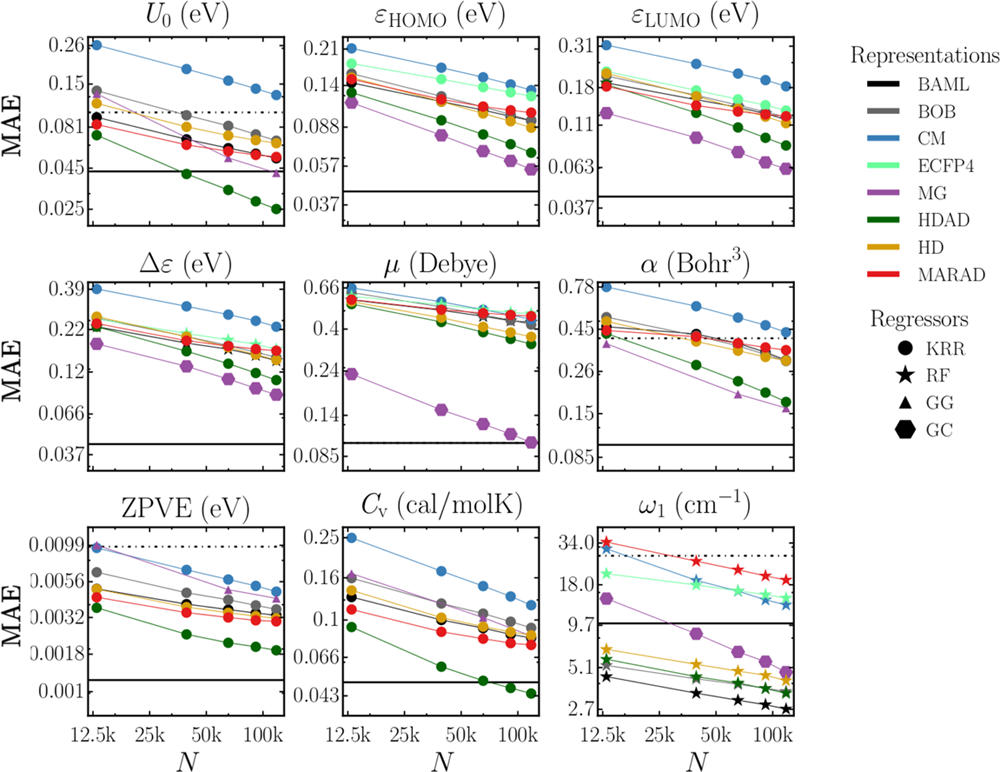
\includegraphics[width=9cm]{linear_and_kernel_models/figures/faber}};
\node[text width=4cm,anchor=east] at (11.5,0) {\small \textit{J. Chem. Theory Comput.} 2017,  13, 11, 5255--5264};
\end{tikzpicture}

\end{frame}
\begin{frame}{KRR example}
jupyter notebook
\end{frame}
